% FILLED (fill batch): process ⑤ Synthesis — pbar+e+ -> Hbar 3-body recomb.
%   folds stdlib recomb_3body_density_power / _exponent / _tratio (PR #1018)
%   + the Mansbach–Keck / Glinsky–O'Neil n_e^2 T^-9/2 scaling + the
%   25^4.5 = 5^9 identity + negative controls, from companion/verify-ledger.json.
\section{Synthesis --- Three-Body Recombination $\bar p + e^+ \to \bar H$}
\label{app:synthesis}

This appendix is the full data record for pipeline process
\textcircled{\scriptsize 5}. We state the dominant three-body
antihydrogen-formation channel and its $n_e^2 T^{-9/2}$ rate scaling, prove
the temperature-ratio identity $25^{4.5}=5^9$, and pair the integer density
power and doubled temperature exponent with \tierBlue\ atoms. Every digit
traces to PR~\#1018 (dimensional) / \#1094 (BLUE-MAX) and the atoms in
\texttt{companion/verify-ledger.json}.

% -------------------------------------------------------------------------
\subsection{The three-body recombination channel and its scaling}
\label{app:synth-deriv}

Once the antiprotons are cold and overlapped with a dense positron plasma,
neutral antihydrogen forms predominantly by \emph{three-body recombination}:
a second positron carries away the binding energy that a two-body radiative
capture would have to emit as a photon,
\begin{equation}
\bar p + e^+ + e^+ \;\longrightarrow\; \bar H + e^+ ,
\label{eq:synth-channel}
\end{equation}
the channel exploited in the early driven-production experiments
\citep{gabrielse2002driven}. The per-antiproton formation rate in the
classical-collisional regime follows the Mansbach--Keck / Glinsky--O'Neil
scaling \citep{glinsky1991oneil}:
\begin{equation}
\boxed{\;\frac{1}{N_{\bar p}}\frac{dN_{\bar H}}{dt}
\;\propto\; n_e^{2}\,T^{-9/2}\;}.
\label{eq:synth-scaling}
\end{equation}
The two exponents carry the physics. The density power $2$ is the
three-body signature: two positrons participate in each capture, so the rate
scales as the positron density \emph{squared}. The temperature power
$-9/2$ is steep --- the rate climbs as $T$ drops, because the recombination
phase space (the volume of weakly-bound Rydberg states accessible to a
collision) grows as the thermal energy falls. Both are exact BLUE-MAX integer
atoms in their natural integer forms (\verb|recomb_3body_density_power|$=2$;
\verb|recomb_3body_exponent_doubled|$=-9$, the doubling clearing the
half-integer; Appendix~\ref{app:bluemax}). The normalized rate scaling
$R(T)/R(4\,\mathrm{K})=(T/4)^{-9/2}$, its registered anchor, and the
discriminating wrong-slope control are plotted in Fig.~\ref{fig:synth-t92}.

\begin{figure}[h]
\centering
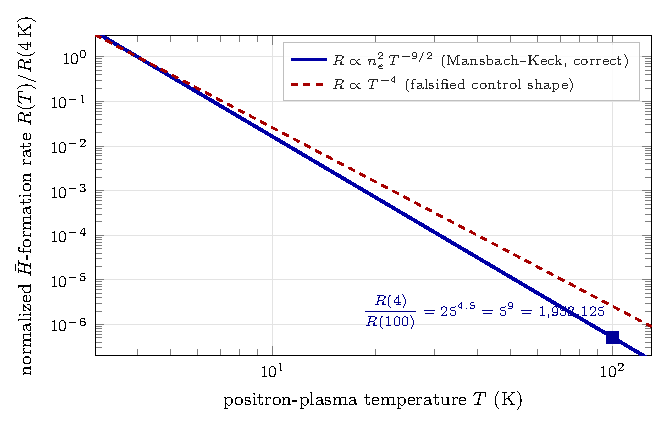
\includegraphics[width=0.82\linewidth]{figures/fig08_recomb_t92.pdf}
\caption{Three-body $\bar H$-formation rate versus positron-plasma
temperature, normalized to $4$\,K at fixed $n_e$ (log--log). The correct
$T^{-9/2}$ scaling (blue) passes exactly through the registered anchor: the
$4$\,K-to-$100$\,K rate ratio is $(100/4)^{9/2}=25^{4.5}=5^9=1{,}953{,}125$
(\texttt{recomb\_3body\_tratio}, PR~\#1018), i.e.\ the marked point
$R(100)/R(4)=1/1{,}953{,}125\approx5.1\times10^{-7}$. The dashed red line is
the implied shape of the falsified $T^{-4}$ control. Only the single
registered ratio anchor is a verify atom; the curves are the exact scaling
laws (commons @D~g3). The steep slope is why production demands the coldest
achievable positron plasma.}
\label{fig:synth-t92}
\end{figure}

% -------------------------------------------------------------------------
\subsection{The $25^{4.5}=5^9$ closed-form identity}
\label{app:synth-identity}

The temperature-ratio atom \verb|recomb_3body_tratio(100,4)| evaluates the
exact rate ratio between a $4$\,K and a $100$\,K plasma:
\begin{equation}
\Bigl(\frac{100}{4}\Bigr)^{9/2}
= 25^{9/2}
= (5^2)^{9/2}
= 5^{9}
= 1{,}953{,}125 ,
\label{eq:synth-id}
\end{equation}
an exact integer despite the half-integer exponent, because $25=5^2$ makes
the $9/2$ power collapse to the integer power $5^9$. This is why the atom
verifies to $|\Delta|=0$ rather than carrying a \texttt{pow} round-off: the
intermediate is an exact integer. A $4$\,K plasma therefore recombines almost
\emph{two million times} faster than a $100$\,K one --- the quantitative
mandate for the deep cooling of process \textcircled{\scriptsize 4}.

\begin{table}[h]
\centering
\small
\setlength{\tabcolsep}{5pt}
\begin{tabular}{@{}l l r r r l@{}}
\toprule
\textbf{atom} & \textbf{args} & \textbf{expected} & \textbf{observed} & $|\Delta|$ & \textbf{tier} \\
\midrule
\verb|recomb_3body_density_power|         & (1)          & $2$        & $2$        & $0$ & \tierBlue \\
\verb|recomb_3body_exponent_doubled|      & ()           & $-9$       & $-9$       & $0$ & \tierBlue \\
\verb|recomb_3body_tratio_exponent_doubled| & ()         & $9$        & $9$        & $0$ & \tierBlue \\
\verb|recomb_3body_exponent|              & ()           & $-4.5$     & $-4.5$     & $0$ & \tierGreen \\
\verb|recomb_3body_tratio|                & (100.0,4.0)  & $1953125.0$& $1953125.0$& $0$ & \tierGreen \\
\bottomrule
\end{tabular}
\caption{Process \textcircled{\scriptsize 5} synthesis atoms
(\texttt{companion/verify-ledger.json}, PR~\#1018 / \#1094). The three
\tierBlue\ integer atoms attest the density power $2$ and the doubled
temperature exponents ($\pm9$); the two \tierGreen\ atoms attest the
half-integer exponent $-4.5$ and the exact ratio
$25^{4.5}=5^9=1{,}953{,}125$.}
\label{tab:synth-verify}
\end{table}

\begin{lstlisting}
verify --expr recomb_3body_tratio(100.0,4.0)=1953125.0
  calc   = 1953125.0 ~ expected 1953125.0 (|Delta|=0.0 <= eps=1e-9)
  tier   = SUPPORTED-NUMERICAL (hexa-native libm-class recompute)
verify --expr recomb_3body_density_power(1)=2
  calc   = 2 == expected 2 (|Delta|=0)
  tier   = SUPPORTED-FORMAL (integer algebraic-root identity)
verify --expr recomb_3body_tratio(100.0,4.0)=2000000.0   # negative control
  calc   = 1953125.0 != expected 2000000.0 (|Delta|=46875 > eps=1e-9)
  tier   = FALSIFIED (controlled negative)
\end{lstlisting}

% -------------------------------------------------------------------------
\subsection{Negative controls}
\label{app:synth-controls}

Three deterministic controls return \textsc{Falsified}: a wrong density power
($3$ instead of $2$), a wrong temperature exponent ($-4.0$ instead of
$-4.5$, the $T^{-4}$ shape of Fig.~\ref{fig:synth-t92}), and a wrong ratio
($2{,}000{,}000$ instead of $1{,}953{,}125$). Each confirms the verifier
distinguishes the correct scaling from nearby wrong powers.

% -------------------------------------------------------------------------
\subsection{Honest scope}
\label{app:synth-scope}

This appendix closes the recombination-rate \emph{scaling}
($\propto n_e^2 T^{-9/2}$) and the exact temperature-ratio identity, not an
absolute $\bar H$-formation rate in $\mathrm{s}^{-1}$. The absolute rate
carries a dimensional prefactor and depends on the positron-plasma density,
overlap volume, and the (eventually flattening) low-$T$ behaviour of the
collisional theory; these are plasma inputs out of scope here. No absolute
rate is claimed or plotted (commons @D~g3).
